%%%%%%%%%%%%
\begin{textblock}{17.5}(4,84)
%\begin{block}{Collaborative Analyses}
{\bf Collaborative Analyses} \\
Establish infrastructure for a higher-level of collaborative analysis, building on the successful patterns used for the Higgs boson discovery and enabling a deeper communication between the theoretical community and the experimental community 
\begin{figure}[tbph]
\centering

\includegraphics[width=1.0\textwidth]{collaborate.png}
\end{figure}
%\end{block}
\end{textblock}

\begin{textblock}{17.5}(23.5,84)
%\begin{block}{Reproducible Analyses}
{\bf Reproducible Analyses} \\
Streamline efforts associated to reproducibility, analysis preservation, and data preservation by making these native concepts in the tools
\begin{figure}[tbph]
\centering

\includegraphics[width=1.0\textwidth]{collaborate.png}
\end{figure}
%\end{block}
\end{textblock}

\begin{textblock}{17.5}(43,84)
%\begin{block}{Interoperability}
{\bf Interoperability} \\
Improve the interoperability of HEP tools with the larger scientific software ecosystem, incorporating best practices and algorithms from other disciplines into HEP
\begin{figure}[tbph]
\centering

\includegraphics[width=1.0\textwidth]{interoperable.png}
\end{figure}
%\end{block}
\end{textblock}

\begin{textblock}{17.5}(62.5,84)
%\begin{block}{Faster Processing}
{\bf Faster Processing} \\
Improve the interoperability of HEP tools with the larger scientific software ecosystem, incorporating best practices and algorithms from other disciplines into HEP
\begin{figure}[tbph]
\centering

\includegraphics[width=1.0\textwidth]{faster-processing.jpg}
\end{figure}
%\end{block}
\end{textblock}

%%%%%%%%%%%%%%%%%%%%%%

%%%%%%%%%%%%
\begin{textblock}{17.5}(4,54)
%\begin{block}{Better Software}
{\bf Better Software} \\
Develop software to effectively exploit emerging many- and multi-core hardware. 
Promote the concept of software as a research product.
\begin{figure}[tbph]
\centering
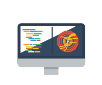
\includegraphics[width=1.0\textwidth]{better-software.png}
\end{figure}
%\end{block}
\end{textblock}

\begin{textblock}{17.5}(23.5,54)
%\begin{block}{Training}
{\bf Training} \\
Provide training for students in all of our core research topics.
\begin{figure}[tbph]
\centering

\includegraphics[width=1.0\textwidth]{training.png}
\end{figure}
%\end{block}
\end{textblock}



